\documentclass[12pt]{article}

% Layout.
\usepackage[top=1in, bottom=0.75in, left=1in, right=1in, headheight=1in, headsep=6pt]{geometry}

% Fonts.
\usepackage{mathptmx}
\usepackage[scaled=0.86]{helvet}
\renewcommand{\emph}[1]{\textsf{\textbf{#1}}}

% TiKZ.
\usepackage{tikz, pgfplots}
\usetikzlibrary{calc}
\pgfplotsset{compat = newest}
 
\pgfplotsset{my style/.append style={axis x line=middle, axis y line=
middle, xlabel={$x$}, ylabel={$y$}, axis equal }}

% Misc packages.
\usepackage{amsmath,amssymb,latexsym}
\usepackage{graphicx}
\usepackage{array}
\usepackage{xcolor}
\usepackage{multicol}

% Commands to set various header/footer components.
\makeatletter
\def\doctitle#1{\gdef\@doctitle{#1}}
\doctitle{Use {\tt\textbackslash doctitle\{MY LABEL\}}.}
\def\docdate#1{\gdef\@docdate{#1}}
\docdate{Use {\tt\textbackslash docdate\{MY DATE\}}.}
\def\doccourse#1{\gdef\@doccourse{#1}}
\let\@doccourse\@empty
\def\docscoring#1{\gdef\@docscoring{#1}}
\let\@docscoring\@empty
\def\docversion#1{\gdef\@docversion{#1}}
\let\@docversion\@empty
\makeatother

% Headers and footers layout.
\makeatletter
\usepackage{fancyhdr}
\pagestyle{fancy}
\fancyhf{} % Clears all headers/footers.
\lhead{\baselineskip 30pt
%\emph{\@doctitle\hfill\@docdate}
\emph{\@docdate\hfill\@doctitle}
\ifnum \value{page} > 1\relax\else\\
\emph{Name: \rule{3.5in}{1pt}\hfill \@docscoring}\fi}
\rfoot{\emph{\@docversion}}
\lfoot{\emph{\@doccourse}}
\cfoot{\emph{\thepage}}
\renewcommand{\headrulewidth}{0pt}%
\makeatother

% Paragraph spacing
\parindent 0pt
\parskip 6pt plus 1pt

% A problem is a section-like command. Use \problem{5} to
% start a problem worth 5 points.
\newcounter{probcount}
\newcounter{subprobcount}
\setcounter{probcount}{0}
\newcommand{\problem}[1]{%
\par
\addvspace{4pt}%
\setcounter{subprobcount}{0}%
\stepcounter{probcount}%
\makebox[0pt][r]{\emph{\arabic{probcount}.}\hskip1ex}\emph{[#1 points]}\hskip1ex}
\newcommand{\thesubproblem}{\emph{\alph{subprobcount}.}}

% Subproblems are an enumerate-like environment with a consistent
% numbering scheme. 
% Use \begin{subproblems}\item...\item...\end{subproblems}
\newenvironment{subproblems}{%
\begin{enumerate}%
\setcounter{enumi}{\value{subprobcount}}%
\renewcommand{\theenumi}{\emph{\alph{enumi}}}}%
{\setcounter{subprobcount}{\value{enumi}}\end{enumerate}}

% Blanks for answers in normal and math mode.
\newcommand{\blank}[1]{\rule{#1}{0.75pt}}
\newcommand{\mblank}[1]{\underline{\hspace{#1}}}
\def\emptybox(#1,#2){\framebox{\parbox[c][#2]{#1}{\rule{0pt}{0pt}}}}

% Misc.
\renewcommand{\d}{\displaystyle}
\newcommand{\ds}{\displaystyle}
\def\bc{\begin{center}}
\def\ec{\end{center}}
\def\be{\begin{enumerate}}
\def\ee{\end{enumerate}}


\doctitle{Math 251: Quiz 8}
\docdate{30 October, 2025}
\doccourse{UAF Calculus I}
\docversion{v-1}
\docscoring{\blank{0.8in} / 25}
\begin{document}
\textbf{Please circle your instructor's name:} \hfill Kevin Meek \hfill James Gossell \hfill Margaret Short \\

There are 25 points possible on this quiz. No aids (book, calculator, etc.)
are permitted.  {\bf Show all work for full credit.}

\problem{11} Let $\displaystyle f(x) = -\frac{1}{10}\left(2x^2\right)\left(x^2-3x\right)$. Note that we have the following:
$$f'(x) = -\frac{1}{10}\left(2x^2\right)\left(4x-9\right)
\hspace{.25in} {\mbox{ and }} \hspace{.24in} f''(x) = -\frac{1}{10}\left(12x\right)\left(2x-3\right)$$
You must show your work for all parts to receive credit!
\begin{subproblems}
\item Determine the intervals where $f$ is increasing and where $f$ is decreasing.
\vfill
\vfill
\item Find the $x$-values where any local maxima occur and where any local minima occur. If none exist, state ``none''.
\vfill
\item Find the intervals where $f$ is concave up and where $f$ is concave down.
\vfill
\vfill
\item Find the $x$-values where any inflection points occur. If none exist, state ``none''.
\vfill
\end{subproblems}

\noindent

\pagebreak

\problem{8} Evaluate the following limits. {\bf{Show your work!}}
\begin{subproblems}
\item
$\displaystyle{\lim_{x \rightarrow \,-\infty}} \,\,
\frac{5x^3-7x^5}{8x^5+10x^4}$

\vfill
\vfill
\item
$\displaystyle{\lim_{x \rightarrow \,-\infty}} \,\,
\frac{3(x^2+8x)}{\sqrt{x^4+2x^2}}$
\vfill
\vfill
\vfill
\end{subproblems}

\problem{6} Based on the graph of the function $g(x)$ below, indicated whether each of the given values is {\bf{positive}}, {\bf{negative}}, {\bf{zero}}, or {\bf{undefined.}}




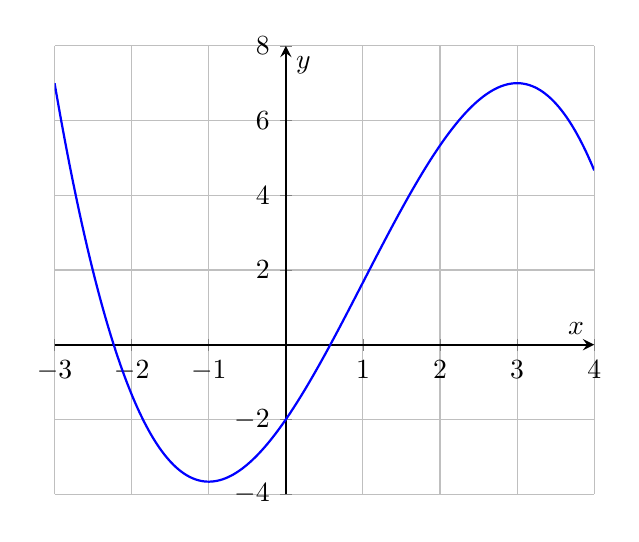
\begin{tikzpicture}
  \begin{axis}[
    axis lines=middle,
    xlabel={$x$},
    ylabel={$y$},
    xmin=-3, xmax=4,
    ymin=-4, ymax=8,
    samples=200,
    domain=-3:4,
    grid=both,
    thick
  ]
    \addplot[
      smooth,
      blue,
      thick
    ]{ -((1/3)*x^3 - x^2 - 3*x) - 2 };
  \end{axis}
\end{tikzpicture}

\begin{multicols}{2}
\begin{subproblems}
\item $g'(-1)$
\vspace{.2in}
\item $g'(0.5)$
\vspace{.2in}
\item $g'(3)$
\vspace{.2in}
\item $g''(-1)$
\vspace{.2in}
\item $g''(0.5)$
\vspace{.2in}
\item $g''(3)$
\vspace{.2in}
\end{subproblems}
\end{multicols}

	
\end{document}
%%% Local Variables:
%%% mode: LaTeX
%%% TeX-master: t
%%% End:
